\documentclass[12pt]{amsart}

\addtolength{\hoffset}{-2.25cm}
\addtolength{\textwidth}{4.5cm}
\addtolength{\voffset}{-2.5cm}
\addtolength{\textheight}{5cm}
\setlength{\parskip}{0pt}
\setlength{\parindent}{15pt}

\usepackage[export]{adjustbox}
\usepackage{listings}
\usepackage{amsthm}
\usepackage{amsmath}
\usepackage{amssymb}
\usepackage[colorlinks = true, linkcolor = black, citecolor = black, final]{hyperref}

\usepackage{graphicx}
\usepackage{multicol}
\usepackage{ marvosym }
\usepackage{wasysym}
\usepackage{tikz}
\usetikzlibrary{patterns}

\newcommand{\ds}{\displaystyle}
\DeclareMathOperator{\sech}{sech}


\setlength{\parindent}{0in}

\pagestyle{empty}

\begin{document}

\thispagestyle{empty}

{{\scshape \large Project 3: Building Networks with Tensorflow and Keras} 

\smallskip 

{COSC 525} \hfill { Su-Ann Chong} \hfill{03-26-2021}

\smallskip

\hrule

\bigskip
\section{Introduction}
% A short introduction to the problem 
In this project, multiple face attribute classifers with different network architectures for images are built. A version of the \href{https://github.com/joojs/fairface}{FairFace dataset} was used to train the networks. The images are converted to grayscale and resized to 32 $\times$ 32 pixels. Each face has 3 different attributes that can be used for classification, namely race, gender and age. In this project, models are trained to classify gender and race of a face. 

\bigskip

Five different architectures were experimented:
\begin{enumerate}
	\item Fully Connected Neural Network
	\item Small Convolutional Neural Network
	\item Convolutional Neural Network
	\item Convolutional Neural Network on Two Tasks Simultaneously
	\item Variational Auto Encoder 
\end{enumerate}

\bigskip

% \pagebreak
\section{Introduction to Each Network Architectures}
\begin{enumerate}

	\item{Task 1: Fully Connected Neural Network} \\

		This architecture consists of all fully connected layers with the following specifications:

		\begin{table}[h]
		\caption{Fully Connected Neural Network Architecture}
		\begin{tabular}{c c c c }
		\hline
		Layer & Type & Number of neurons & Activation Function \\
		\hline
		1 & Flatten & - & - \\
		2 & Dense & 1024 & "tanh" \\
		3 & Dense & 512 & "sigmoid" \\
		4 & Dense & 100 & "relu" \\
		5 & Dense & n - number of classes & "softmax" \\
		\hline 
		\end{tabular}
		\end{table}

	\item{Task 2: Small Convolutional Neural Network} \\

		This architecture consists of layers with the following specifications:

		\begin{table}[h]
		\caption{Small Convolutional Neural Network Architecture}
		\begin{tabular}{c c c c c c c}
		\hline
		Layer & Type & Number of neurons & Stride & Padding & Activation Function & Pool size\\
		\hline
		1 & Conv2D & 5 $\times$ 5 $\times$ 40 & 1 & "valid" & "relu" & -\\
		2 & MaxPooling2D & - & - & - & - & 2\\
		3 & Flatten & - & - & - & - & - \\
		4 & Dense & 100 & - & - & "relu" & - \\
		5 & Dense & n - number of classes & - & - & "softmax" & - \\
		\hline 
		\end{tabular}
		\end{table}
\vfill

\pagebreak
	\item{Task 3: Convolutional Neural Network} \\
		This architecture consists of layers with the following specifications:

		\begin{table}[h]
		\caption{Convolutional Neural Network Architecture}
		\begin{tabular}{c c c c c c c c}
		\hline
		Layer & Type & Number of neurons & Stride & Padding & Activation function & Pool size\\
		\hline
		1 & Conv2D & 3 $\times$ 3 $\times$ 32 & 1 & "same" & "relu" & - \\
		2 & Conv2D & 3 $\times$ 3 $\times$ 32 & 1 & "same" & "relu" & -\\
		3 & MaxPooling2D & - & - & - & - & 2\\
		 & Dropout 0.25 & - & - & - & - & -\\
		4 & Conv2D & 3 $\times$ 3 $\times$ 64 & 1 & "same" & "relu" & - \\
		5 & Conv2D & 3 $\times$ 3 $\times$ 64 & 1 & "same" & "relu" & - \\
		6 & MaxPooling2D & - & - & - & - & 2\\
		& Dropout 0.25 & - & - & - & - & -\\
		7 & Flatten & - & - & - & - & -\\
		8 & Dense & 512 & - & - & "relu" & -\\
		& Dropout 0.5 & - & - & - & - & -\\
		9 & Dense & n - number of classes & - & - & "softmax" & -\\
		\hline 
		\end{tabular}
		\end{table}

	\item{Task 4: Multi-task Convolutional Neural Network} \\

		This architecture consists of layers with the following specifications:

		\begin{table}[h]
		\caption{Multi-task Convolutional Neural Network Architecture}
		\begin{tabular}{c c c c c c c c}
		\hline
		Layer & Type & Number of neurons & Stride & Padding & Activation function & Pool size\\
		\hline
		1 & Conv2D & 7 $\times$ 7 $\times$ 32 & 1 & "same" & "relu" & - \\
		2 & MaxPooling2D & - & 2 & "same" & - & 3\\
		3 & Lambda & - & - & - & - & -\\

		4 & Conv2D & 1 $\times$ 1 $\times$ 64 & 1 & "same" & "relu" & - \\
		5 & Conv2D & 3 $\times$ 3 $\times$ 192 & 1 & "same" & "relu" & - \\
		6 & MaxPooling2D & - & - & - & - & 2\\
		7 & Lambda$^{\dagger}$ & - & - & - & - & -\\
		% (local response normalization) \\
		8 & Flatten & - & - & - & - & -\\
		9 (1) & Dense & 100 & - & - & "relu" & -\\
		9 (2) & Dense & 100 & - & - & "relu" & -\\
		10 (1) & Dense & n - number of classes & - & - & "softmax" & -\\
		10 (2) & Dense & n - number of classes & - & - & "softmax" & -\\
		\hline 
		\end{tabular}
		\end{table}

		$^{\dagger}$ This Lambda layer is the local response normalization function. 

		\vfill
		\pagebreak

	\item{Task 5: Variational Auto Encoder} \\

		This architecture consists of layers with the following specifications: \\

		\begin{table}[h]
		\caption{Encoder Network Architecture}
		\begin{tabular}{c c c c c c c c}
		\hline
		Layer & Type & Number of neurons & Stride & Padding & Activation function & Pool size\\
		\hline
		1 & Conv2D & 7 $\times$ 7 $\times$ 16 & 1 & "same" & "relu" & - \\
		2 & Conv2D & 3 $\times$ 3 $\times$ 32 & 1 & "same" & "relu" & - \\
		3 & Flatten & - & - & - & - & -\\
		4 & Dense & 32 & - & - & "relu" & -\\
		5 (1) & Dense & latent dimension & - & - & - & - \\
		5 (2) & Dense & latent dimension & - & - & - & -\\
		6 & Lambda  & - & - & - & - & -\\
		\hline 
		\end{tabular}
		\end{table}

		$^{\dagger}$ This Lambda layer is the local response normalization function.

		\begin{table}[h]
		\caption{Decoder Network Architecture}
		\begin{tabular}{c c c c c c c c}
		\hline
		Layer & Type & Number of neurons & Stride & Padding & Activation function & Pool size\\
		\hline
		1 & Dense & 32 $\times$ 32 $\times$ 32 & - & - & "relu" & -\\
		2 & Reshape & - & - & - & - & - \\
		3 & Conv2DTranspose & 3 $\times$ 3 $\times$ 32 & 1 & "same" & "relu" & - \\
		4 & Conv2DTranspose & 7 $\times$ 7 $\times$ 16 & 1 & "same" & 
		"relu" & - \\
		5 & Conv2DTranspose & 3 $\times$ 3 $\times$ 1 & 1 & "same" & "relu" & - \\
		\hline 
		\end{tabular}
		\end{table}

		$^{\dagger}$ This Lambda layer is the local response normalization function.

\end{enumerate}

\section{Results of Each Network Architecture} 

	Here is a summary of parameters used for each network and the accuracy obtained:

	\begin{table}[h]
	\begin{tabular}{r c c c c c c c} 
	\hline
	Task & type & learning rate & momentum & batch size & epoch & loss function & accuracy(\%) \\
	\hline
	1 & gender & 0.001 & 0.9 & 32 & 50 & categorical cross entropy & 75.04 \\
	
	2 & gender & 0.001 & 0.9 & 32 & 50 & categorical cross entropy & 79.66 \\
	
	3 & gender & 0.001 & 0.9 & 32 & 25 & categorical cross entropy & 81.96\\
	
	4 & gender & 0.001 & 0.9 & 32 & 30 & categorical cross entropy & 81.81 \\
	\hline
	\end{tabular}
	\end{table}

	\begin{table}[h]
	\begin{tabular}{r c c c c c c c} 
	\hline
	Task & type & learning rate & momentum & batch size & epoch & loss function & accuracy(\%) \\
	\hline
	1& race  & 0.001 & 0.9 & 32 & 50 & categorical cross entropy & 43.10 \\
	2& race  & 0.001 & 0.9 & 32 & 50 & categorical cross entropy & 46.61\\
	3& race  & 0.001 & 0.9 & 32 & 25 & categorical cross entropy & 52.39 \\
	4& race  & 0.001 & 0.9 & 32 & 30 & categorical cross entropy & 51.24 \\
	% \hline
	% \end{tabular}
	% \end{table}

	% \begin{table}[h]
	% \begin{tabular}{r c c c c c c c} 
	% \hline
	% Task & type & learning rate & momentum & batch size & epoch & loss function & accuracy(\%) \\
	% \hline
	5 & - & 0.001 & 0.9 & 256 & 50 & mean squared error & - \\
	\hline
	\end{tabular}
	\end{table}

	\vfill 

	\begin{enumerate}
	\item Fully Connected Neural Network \\

	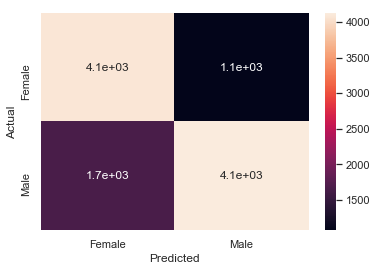
\includegraphics[width=0.48\textwidth]{task1g_cm} 
	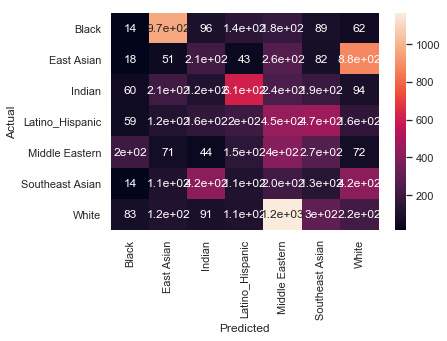
\includegraphics[width=0.48\textwidth]{task1r_cm}  
	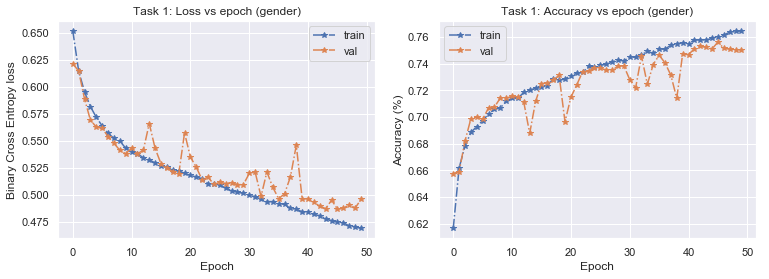
\includegraphics[width=\textwidth]{task1g_plots}
	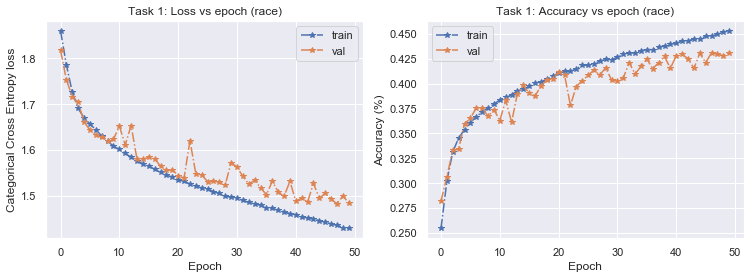
\includegraphics[width=\textwidth]{task1r_plots}
	
	\vfill 

	\item Small Convolutional Neural Network \\

	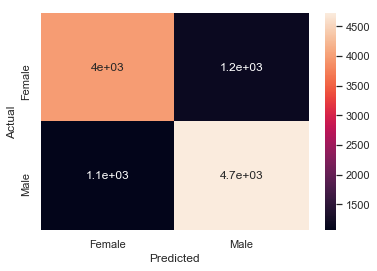
\includegraphics[width=0.48\textwidth]{task2g_cm} 
	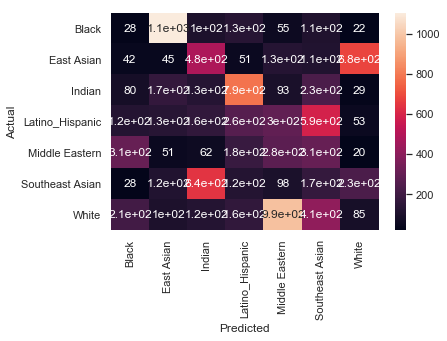
\includegraphics[width=0.48\textwidth]{task2r_cm} 
	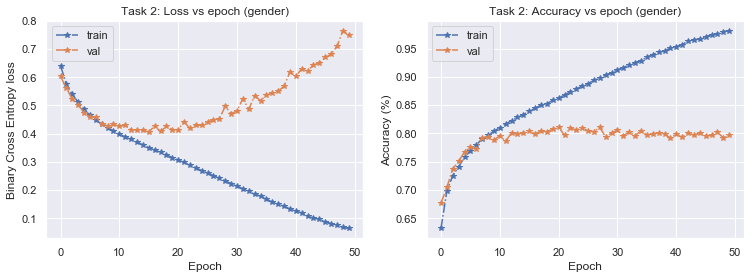
\includegraphics[width=\textwidth]{task2g_plots}
	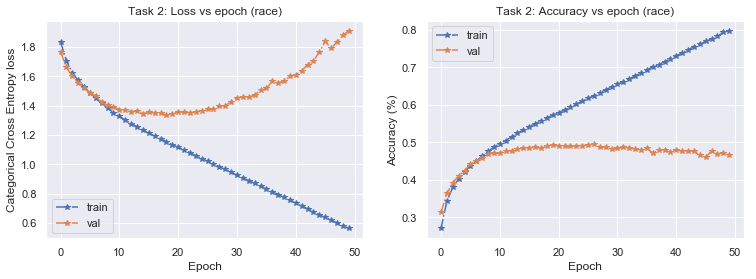
\includegraphics[width=\textwidth]{task2r_plots}

	\vfill 

	\item Convolutional Neural Network \\

	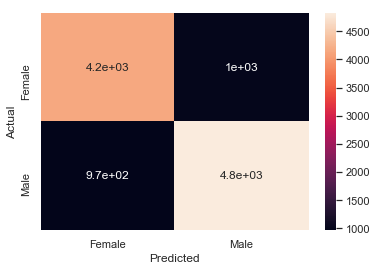
\includegraphics[width=0.48\textwidth]{task3g_cm} 
	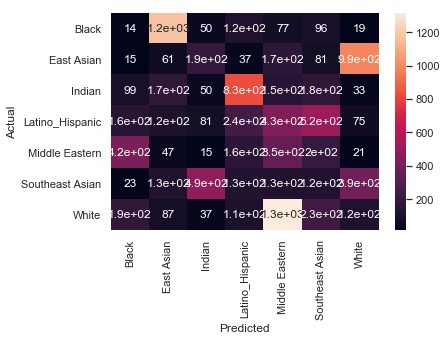
\includegraphics[width=0.48\textwidth]{task3r_cm} 
	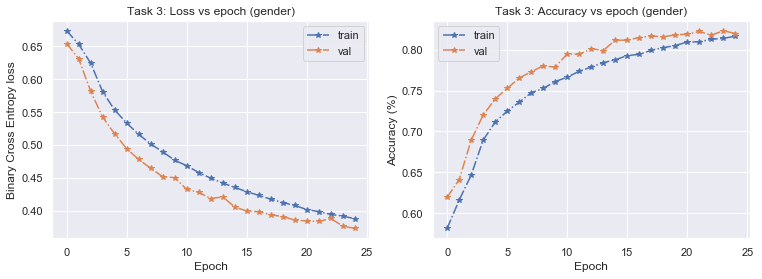
\includegraphics[width=\textwidth]{task3g_plots}
	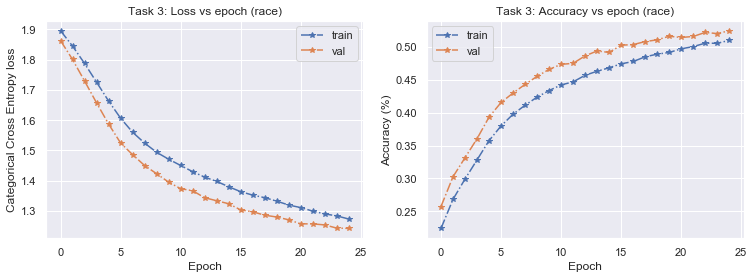
\includegraphics[width=\textwidth]{task3r_plots}

	\vfill 

	\item Convolutional Neural Network on Two Tasks Simultaneously \\

	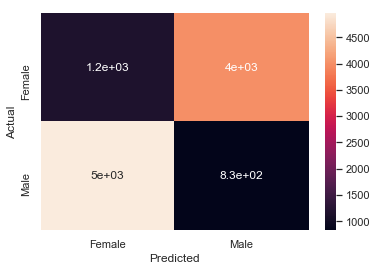
\includegraphics[width=0.48\textwidth]{task4g_cm} 
	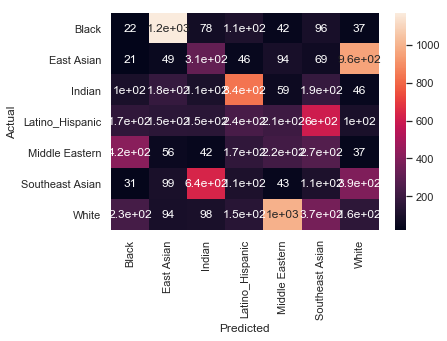
\includegraphics[width=0.48\textwidth]{task4r_cm} 
	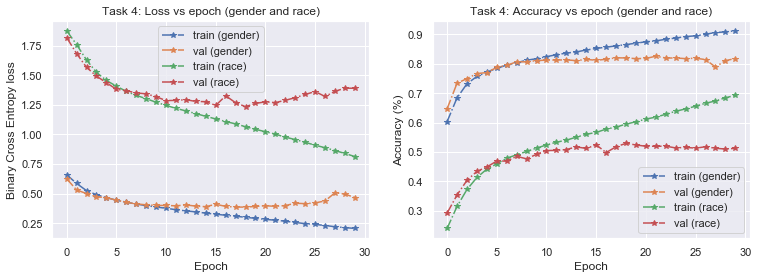
\includegraphics[width=\textwidth]{task4_plots}

	\vfill 

	\item Variational Auto Encoder 

	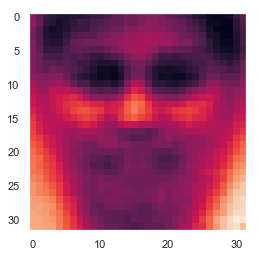
\includegraphics[width=0.48\textwidth]{task5_1} 
	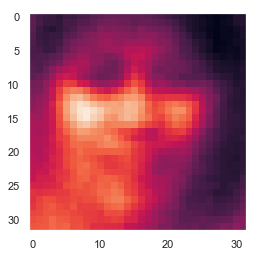
\includegraphics[width=0.48\textwidth]{task5_2} 
	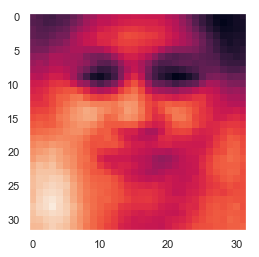
\includegraphics[width=0.48\textwidth]{task5_3} 
	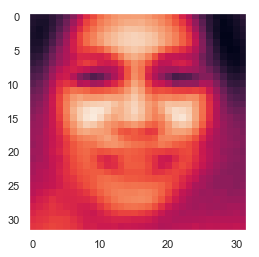
\includegraphics[width=0.48\textwidth]{task5_4} 
	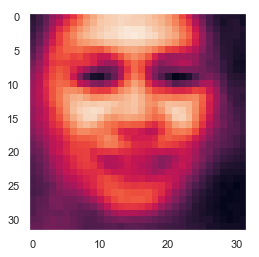
\includegraphics[width=0.48\textwidth]{task5_5} 
	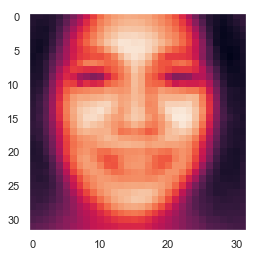
\includegraphics[width=0.48\textwidth]{task5_6} 
	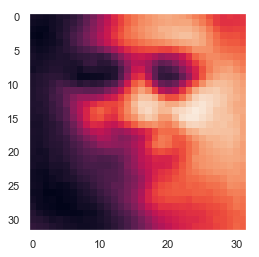
\includegraphics[width=0.48\textwidth]{task5_7} 
	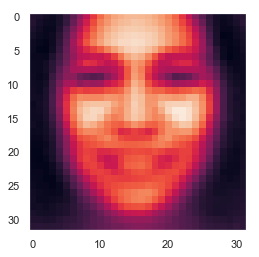
\includegraphics[width=0.48\textwidth]{task5_8} 
	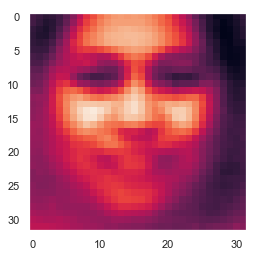
\includegraphics[width=0.48\textwidth]{task5_9} 
	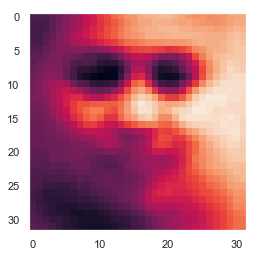
\includegraphics[width=0.48\textwidth]{task5_10} 
	\end{enumerate}


\section{Conclusion}
\begin{itemize}

	\item Convolutional neural networks (Task 2) performs better in classifying image dataset than fully connected networks (Task 1) in both tasks. 
%
	\item Deeper convolutional neural networks (Task 3) give better accuracy than shallower convolutional neural network (Task 2) and are less proned to overfitting. 

	\item Multi-task convolutional neural networks (Task 4) have comparable performance when compared to single-task convolutional neural networks. Overfitting of the training data is observed.

	\item The variational autoencoder model (Task 5) is capable of picking up important features of the faces but the produced images are a lot blurrier than the original images. Training for longer may produce better result if more computing resources is available.

\end{itemize}

\section{How to run code}
You can run the project code with examples using the following command:
\begin{lstlisting}[language=bash]
$ python proj3.py task[1-5]
\end{lstlisting}

\end{document}